\chapter{Arkitektur}
Dette afsnit beskriver de valg, der er blevet foretaget ifht. arkitekturen bag BargainBarter. Der vil kort blive redegjort for de enkelte begreber og arkitekturstile, der blev anvendt til at opbygge systemet. Dernæst følger en analyse af domænet, der ligger til grund for systemets videre design. \\ 

\noindent Der blev i kravspecifikationen i afsnit \ref{ch:Krav} stillet nogle krav til systemet. På baggrund af kravene skulle der udvikles en webapplikation med en tilknyttet database. Webapplaktionen skulle have mulighed for at skaleres til andre platforme. \\

\noindent I de følgende afsnit vil de specifikke teknologier, der er anvendt i projektet, til at opfylde projektets krav.

\section{ASP.NET MVC}
Frameworket ASP.NET MVC\cite{MVC} fra Microsoft blev valgt som platform til webapplikationen, da dette framework opfylder kravene til projektet. Gruppen synes det kunne være en interessant teknologi at arbejde med, og det bliver brugt i vidt omfang i industrien. Desuden har frameworket mange fordele i forhold til udviklingen af projektet: 
\begin{enumerate}
	\item ASP.NET MVC understøtter .NET frameworket, hvilket muliggør udvikling i C\#.
	\item Frameworket har eksisteret i mange år og er derfor veldokumenteret og mange biblioteker understøtter dette framework.
	\item Gruppen har modtaget undervisning i ASP.NET MVC i forbindelse med faget I4GUI.
\end{enumerate}
Der er en masse andre framework, der kunne have været interessante at anvende, såsom Ruby on Rails. Men disse framework understøtter ikke .NET eller C\#, hvilket var vigtigt for gruppen. \\


\noindent På figur \ref{fig:MVC} kan den overordnede struktur af ASP.NET MVC ses.\footnote{Inspireret af PER's slides til lektion 24 i I4GUI 2016}
\begin{figure}[H]
	\centering
	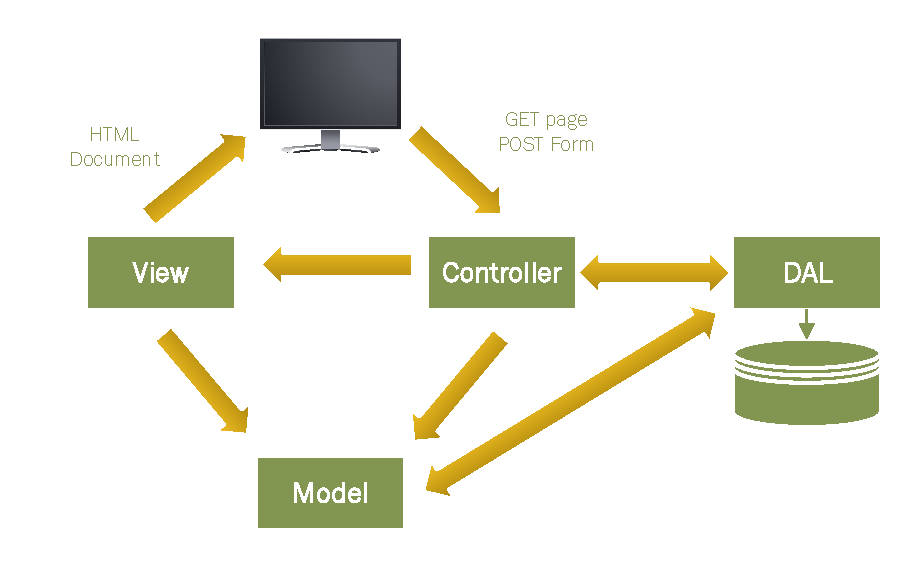
\includegraphics
	[width=140mm]{figures/MVC_drawing.pdf}
	\caption{MVC struktur}
	\label{fig:MVC}
\end{figure}
 \noindent ASP.NET MVC er udviklet på baggrund af 3-lagsmodellen\cite{3-Layer}. 3-lagsmodellen er en client-server arkitekturstil, som sørger lav kobling mellem lagene i systemet. Dette gør systemet skalerbart og vedligeholdelsesvenligt. Modellen består af følgende tre lag:
 \begin{enumerate}
 	\item En front-end web-server der leverer statisk eller dynamisk materiale - dvs. al det materiale der vises i webbrowseren.
 	\item Et lag der generer og processerer dynamisk materiale.
 	\item En back-end database til at gemme og hente data fra.
 \end{enumerate}
 For yderligere information henvises der til dokumentation. \footnote{Se bilag - Dokumentation, sektion 8}\\ 
 
  
 \noindent Nedenunder ses ansvarsområderne for de forskellige dele af ASP.NET MVC. For en uddybende beskrivelse af MVC henvises til dokumentationen \footnote{Se bilag - Dokumentation, sektion 8}.

\begin{itemize}
	\item Model er den del der arbejder med den data relaterede logik, dvs. Data Acces Layer. Det er altså al den data der tages fra databasen og bliver manipuleret af Views eller Controllers.
	\item View er præsentationslogikken. 
	\item Controller er bindeleddet mellem Model og Views. Dens opgave er at manipulere data fra modellen og interagere med Views for at vise outputtet og modtage inputs fra viewet. Businesslogikken er hovedsagligt tilknyttet controllers.
\end{itemize}


\subsection{Data access layer}
I forbindelse med databasetilgangen og brugen blev Entity Framework(EF)\cite{ADOEF} anvendt. Entity framework  var det oplagte valg, på baggrund af valget om at benytte ASP.NET MVC. EF kommer som standard, når der oprettes et ASP.NET MVC projekt, og opretter selv en skabelon til at oprette database tabeller. EF er et object-relational mapping (ORM) framework til ADO.NET, der understøtter udviklingen af dataorienterede applikationer. Det vil sige, at EF sørger for en bekvemmelig og ensartet tilgang til den database man anvender til at gemme og hente data til viewet.  Dette gør EF ved at fjerne impedans mismatchet i mellem databasen og koden. Hertil kommer, at gruppen har fået undervisning i I4DAB, og desuden er EF bekvemt, da gruppen er vant til objektorienteret programmering.\\
 \noindent Til selve databasen er der anvendt SQL Server 2016, som IHA har stillet til rådighed.
 
\subsection{Presentation layer}
Til præsentationslaget anvendes der HTML og CSS til at præsentere data for brugeren. Da brugervenlighed var centralt for systemet blev Bootstrap\cite{Bootstrap} anvendt. Bootstrap er et framework, der gør webapplikationen responsiv og skalerbar. Frameworket gør det nemt at designe et View, der kan skaleres til en hvilken som helst skærm - uanset om det er mobil, tablet eller desktop. Desuden indeholder Bootstrap en række temaer/templates, der gør det enkelt at designe et pænt View. \\
For at gøre View'et mere dynamisk er der flere steder anvendt Javascript og JQuery\cite{jQuery}. 
JQuery gør det muligt f.eks. at vise popup vinduer, der er anvendt i projektet.

\subsection{Business layer}
Businesslaget er server-side-logikken, som er skrevet i C\#. 

\section{Domæneanalysen}

På figur \ref{fig:Domaneanalyse} ses domæneanalysen af BargainBarter. Denne analyse er lavet på baggrund af de definerede user stories som kan findes i dokumentationen\footnote{Se bilag - Dokumentation, sektion 3.2}. Domæneanalysen er det første overordnede figur af hvordan systemet skal opbygges. Den indeholder afgørende valg for systemets overordnede struktur, og giver gruppen en fælles forståelse af domænet. I domæneanalysen identificeres systemets konceptuelle klasser og deres grænseflader. De konceptuelle klasser ligger til grund for designfasen.
\begin{figure}[H]
	\centering
	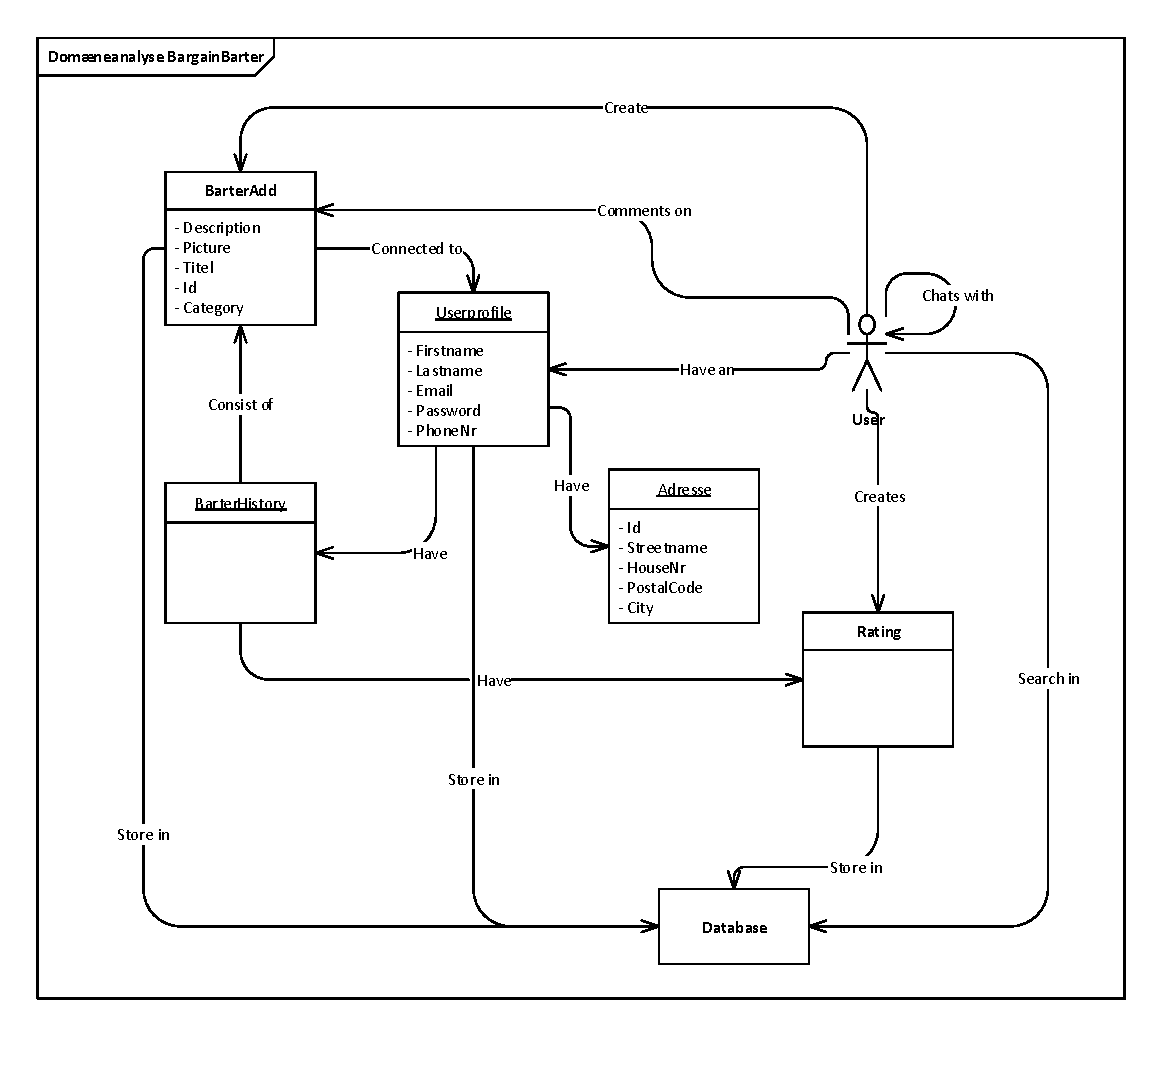
\includegraphics
	[width=140mm]{../Dokumentation/figures/DomaeneanalyseBargainBarter.pdf}
	\caption{Domæneanalyse for BargainBarter}
	\label{fig:Domaneanalyse}
\end{figure}